% !TEX encoding = UTF-8
% !TEX TS-program = pdflatex
% !TEX root = computabilità e algoritmi.tex
% !TEX spellcheck = it-IT
\chapter{Lezione 2}
\section{Introduzione e Algoritmi sui grafi}\label{lezione-2---introduzione-e-algoritmi-sui-grafi}

C'è la possibilità di fare un pre-orale nella settimana dei compitini.

Libro: Cormen, Introduzione agli algoritmi e strutture dati
\href{http://catalogo.unipd.it/F/FCKK1DACESL2TDH5CF15FLDL2BUM936U1XG9U15MFDCKI764BV-10675?func=full-set-set\&set_number=011139\&set_entry=000001\&format=999}{BIB}:

\begin{itemize}
\tightlist
\item
  Introduzione agli algoritmi sui grafi

  \begin{itemize}
  \tightlist
  \item
    Strutture dati per i grafi
  \item
    Operazioni elementari sui grafi
  \end{itemize}
\item
  Algoritmi su stringhe (capitolo 22)
\item
  Algoritmi paralleli (capitolo 27)
\item
  Algoritmi di geometria computazionale
\end{itemize}

\subsection{Terminologia dei grafi}\label{terminologia-dei-grafi}

Un grafo \emph{G} è costituito da un insieme di vertici \emph{V} e di
archi \emph{E}. Ad ogni arco vengono associati due vertici in \emph{V}.

Se c'è un ordine tra i due estremi degli archi, il grafo prende il nome
di \textbf{orientato} o \textbf{diretto}. In questo caso, il primo
vertice prende il nome di \textbf{coda} e l'ultimo \textbf{testa}.

Un \textbf{cappio} è un grafo i cui due estremi coincidono.

Un grafo non orientato si dice \textbf{semplice} se non ha cappi e non
ci sono due archi con gli stessi estremi. Mentre se il grafo è
orientato, perché sia semplice non devono esserci archi con gli stessi
estremi, iniziali e finali. Un grafo non semplice prende il nome di
\textbf{multi-grafo}.

\begin{figure}[htbp]
\centering
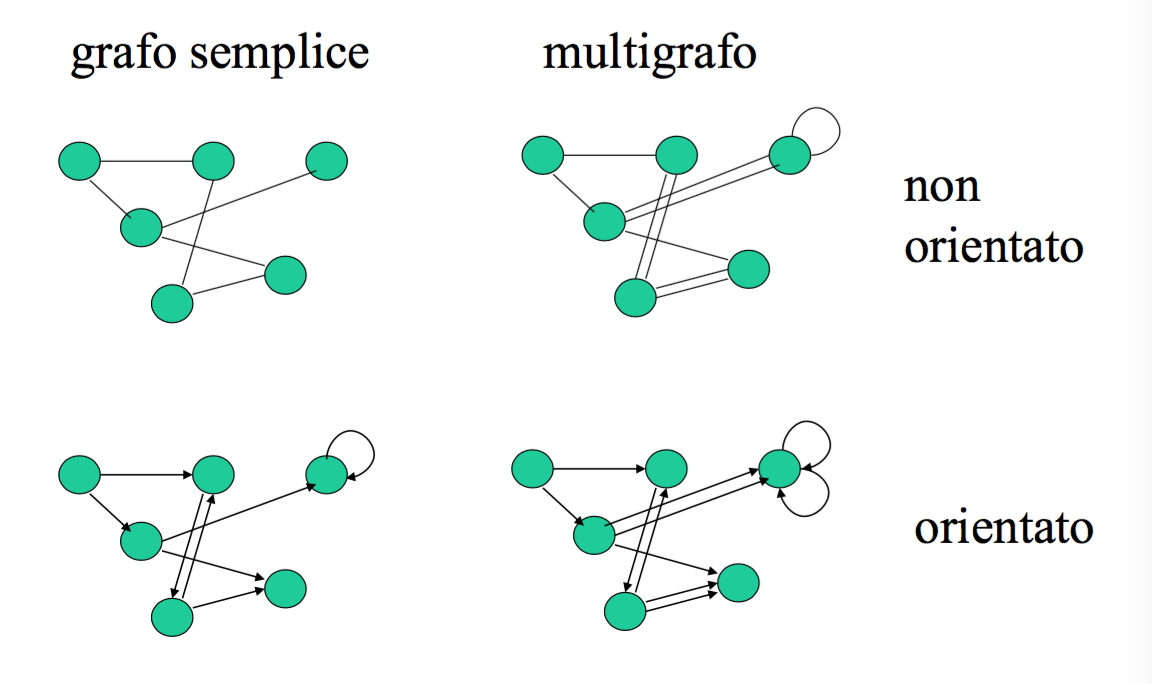
\includegraphics[width=0.75\textwidth]{./notes/immagini/l2-grafi.png}
\caption{Varie tipologie di grafi}
\end{figure}

Se un grafo è semplice, un arco può essere espresso con:

$$
e = uv \in E \text{, con} u,v \in V
$$

e si dice che l'arco \emph{e} è incidente in \emph{u} e \emph{v}. Da
notare che se il grafo è orientato
$e = uv \neq vu$ e la terminologia diventa
``l'arco \emph{e} esce da \emph{u} entra in \emph{v}''.

Il \textbf{grado} di un vertice \emph{v} viene indicato con $\delta(v)$ e rappresenta il numero di archi incidenti in quel
vertice. Se il grafo è ordinato, il suo \textbf{grado uscente} $\delta^+(v)$ è il numero di archi uscenti e il suo \textbf{grado entrante} è $\delta^-(v)$.

Se due vertici sono collegati da un arco, questi vengono detti
\textbf{adiacenti}.

Un \textbf{cammino} di lunghezza \emph{k} da un vertice \emph{u} ad un
vertice \emph{v} in un grafo \emph{G=(V,E)}, è una sequenza di
\emph{k+1} vertici $x_0 \ldots x_k$, tali che $x_0 = u$, $x_k = v$ e $x_{i-1}x_i \in E \forall i = 1\ldots k$.

Se il cammino ha lunghezza 0, questo viene detto \textbf{nullo}, mentre
se il vertice di partenza coincide con quello di arrivo, il cammino
prende il nome di \textbf{chiuso}.

Un cammino viene detto \textbf{semplice} quanto tutti i vertici che lo
compongono sono distinti, ad eccezione del primo, che può coincidere
con l'ultimo. Un cammino semplice e il primo vertice coincide con
l'ultimo, questo prende il nome di \textbf{ciclo}. L'esempio più
semplice di ciclo è dato da un cappio.

Un grafo \textbf{aciclico} è un grafo che non contiene cicli.

Quando esiste almeno un cammino dal vertice \emph{u} al vertice
\emph{v}, si dice che \emph{v} è \textbf{accessibile} (o
\textbf{raggiungibile}) da \emph{u}. Questa definizione è simmetrica
solamente nel caso di un grafo non orientato.

Un grafo non orientato si dice \textbf{connesso} se esiste almeno un
cammino tra ogni coppia di vertici.

Le \textbf{componenti connesse} di un grafo sono le classi di
equivalenza dei suoi vertici rispetto alla relazione di accessibilità,
ovvero un sottoinsieme di vertici che sono tutti tra loro accessibili.

Nel caso di un grafo orientato, si dice che è \textbf{fortemente
connesso} se esiste almeno un cammino tra ogni vertice del grafo. In
modo analogo è possibile definire le \textbf{componenti fortemente
connesse}

Sia la \textbf{connessione} che la \textbf{connessione forte} hanno le
proprietà:

\begin{itemize}
\item
  \textbf{riflessiva}: se c'è una connessione tra \emph{u} e \emph{v},
  c'è anche tra \emph{v} e \emph{u}
\item
  \textbf{transitiva}: se c'è una connessione tra \emph{u} e \emph{v} e
  tra \emph{v} e \emph{z}, allora c'è anche tra \emph{u} e \emph{z}.
\end{itemize}

Un sotto-grafo del grafo \emph{G=(V,E)} è un grafo \emph{G' = (V', E')}
tale che:

$$
V' \subseteq V \: \text{e} \: E' \subseteq \{ uv : uv \in E \text{ e } u,v \in V' \}
$$

ovvero un grafo che ha alcuni vertici e alcuni archi del grafo iniziale.
Da notare che se tolgo un vertice, devo togliere anche tutti gli archi
incidenti in quel vertice.

Se il sotto-grafo viene ottenuto rimuovendo solo dei vertici, questo
prende il nome di \textbf{indotto}, perché la rimozione degli archi
viene forzata dalla rimozione dei vertici.

\subsection{Rappresentazione dei
grafi}\label{rappresentazione-dei-grafi}

Per rappresentare i grafi in un calcolatore è possibile utilizzare la
matrice delle adiacenze o la lista delle adiacenze.

\begin{figure}[htbp]
\centering
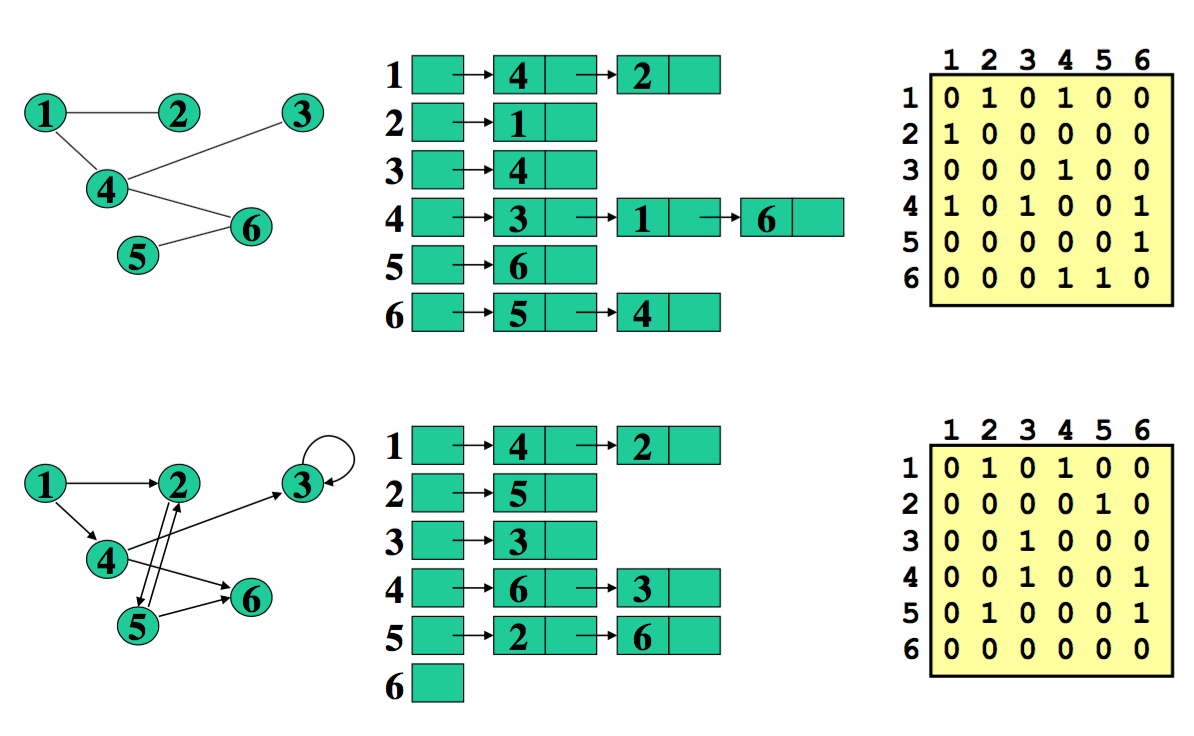
\includegraphics[width=0.75\textwidth]{./notes/immagini/l2-rappr.png}
\caption{Rappresentazione dei grafi}
\end{figure}

\subsubsection{~Lista delle adiacenze}\label{lista-delle-adiacenze}

Per ogni vertice del grafo viene tenuta in memoria una lista \textit{Adj} dei vertici
adiacenti al vertice:

$$
Adj[u] = \{v | uv \in E\} \: \forall u \in V 
$$

Questa rappresentazione richiede memoria per:

\begin{itemize}
\tightlist
\item
  \textit{n\ =\ \textbar{}V\textbar{}} puntatori alla cima delle liste
\item
  \textit{m\ =\ \textbar{}E\textbar{}} elementi per le liste (in totale)
  se il grafo orientato, se è non orientato è \textit{2m}.
\end{itemize}

\subsubsection{Matrice delle adiacenze}\label{matrice-delle-adiacenze}

Viene utilizzata una matrice booleana quadrata che tante righe e tante
colonne, quanti sono i vertici del grafo.

Ogni elemento della matrice vale 1 se i due vertici sono adiacenti, 0
altrimenti:

$$
a_{u,v} = 1 \text{ se } uv \in E
$$

Se il grafo è non orientato, la matrice delle adiacenze è simmetrica.

Il consumo di memoria è $n^2$.

Se il grafo è \textbf{sparso}, ovvero il grado dei vertici è minore del
logaritmo del numero dei vertici, la matrice delle adiacenze risulta
peggiore della rappresentazione con liste in termini di memoria
occupata.

Più formalmente, assumendo che il grafo abbia \textit{n} vertici e \textit{m} archi e che, sia i puntatori, sia gli interi, occupino 32 bit.

Si ha che la lista delle adiacenze occupa $32(n+2m)$, mentre la matrice richiede $n^2$.

La matrice risulta quindi vantaggiosa quando:

\begin{align*}
	32(n+2m) &< n^2 \\
	m &< \frac{n(n-32)}{64}
\end{align*}


\subsection{Calcolo del grafo trasposto}\label{calcolo-del-grafo-trasposto}

Dato un grafo orientato \emph{G=(V,E)} si vuole ottenere $ G^T = (V, E^T)$ in modo che gli archi siano rovesciati, ovvero $E^T = \{uv | vu \in E\}$.

Utilizzando la rappresentazione con la matrice delle adiacenze, è
necessario attraversare metà della matrice e mettere a 1 la cella
\emph{i,j} se \emph{j,i} è a 1. La complessità risulta quindi essere
$O(n^2)$.

Con la lista delle adiacenze l'algoritmo risulta essere


\begin{algorithm}
	\begin{algorithmic}
		\Function{Trasponi}{$Adj,\: Adj^T,\: n$}
			\For{$v = 1 \: to \: n$}
				\State $Adj^T[v] \gets nil$
			\EndFor
			\For{$u = 1 \: to \: n$}
				\State {$x \gets Adj[u]$}
				\While{$x \neq nil$}
					\State{$v \gets x.v$}
					\State{$y \gets nodo(u, Adj^T[v])$}
					\State{$Adj^T[v] \gets y$}
				\EndWhile
			\EndFor
		\EndFunction
	\end{algorithmic}
	\caption{Calcolo del grafo trasposto utilizzando la rappresentazione con la lista delle adiacenze}
\end{algorithm}

Ovvero viene attraversata la lista delle adiacenze del grafo originale,
e per ogni elemento delle liste, lo aggiunge ``\emph{al contrario}''
nella nuova lista delle adiacenze.

La complessità risulta quindi essere \emph{O(m+n)}, questo perché il
secondo \texttt{for} esamina tutti i possibili archi, quindi anziché
avere complessità \emph{n} (numero di vertici) ha complessità \emph{m}
(numero di archi).

\subsection{(Esercizio) Ricerca del pozzo
universale}\label{esericizio-ricerca-del-pozzo-universale}

Un vertice è un \textbf{pozzo universale} se può essere raggiunto da
tutti gli altri vertici del grafo, dal quale però non è possibile
raggiungere altri vertici.

Trovare un algoritmo che riesce a risolvere il problema in \emph{O(n)}.
